\chapter{Iterations 1 and 2: Design and Implementation}
\label{chap:iter1}

\section{Iteration Objectives}
The primary objective of Iterations 1 and 2 (Weeks 1 through 10) was transitioning Project FORGE from an exploratory proof-of-concept into a robust, literature-grounded, and visually polished mid-term deliverable. In direct alignment with the FYP Committee's directives and the FAST School of Computing CI/CD mandate, our goals were:
\begin{enumerate}
    \item \textbf{Commercial Aesthetic Elevation:} Replace all placeholder geometric shapes with 2D pixel-art sprites, integrate trauma-decay camera shake, and deploy color-coded floating combat text.
    \item \textbf{Combat Dynamics Variety:} Implement distinct adversary behavioral archetypes (Melee Crawler and Ranged Pyromancer with telegraphed projectiles) counterbalanced by a player dodge roll with invulnerability frames.
    \item \textbf{Cold-Start Calibration Protocol:} Implement a 5-floor calibration sequence that summarizes the player as an Initial Combat Rating ($CR_0$) and seeds the PPO policy's first observation, avoiding an arbitrary starting difficulty.
    \item \textbf{Non-Adaptive Comparative Baseline:} Provide an in-engine toggle for a deterministic static roguelike baseline to benchmark adaptive generation against standard game pacing.
    \item \textbf{Automated Continuous Integration Solvability Pipeline:} Deploy a GitHub Actions workflow running headless Godot 4.7.2 checks (script loading, a reachability regression test and GDScript tests) on every push to the main branches and every pull request.
\end{enumerate}

\section{Selected Use Cases and Feature Scope}
The implementation completed during this stage satisfies the three core use cases baselined in Chapter~\ref{chap:reqs}:
\begin{itemize}
    \item \textbf{UC-01 (Play Adaptive Session with Cold-Start Calibration):} Implemented across Floors 1 through 5 with the transition into closed-loop PPO generation at Floor 6; the calibration-to-PPO hand-off is covered by headless test TC-02.
    \item \textbf{UC-02 (Combat Encounters and Tactical Evasion):} Fully realized with dynamic melee/ranged combat, projectile kinematics, collision detection, and player dodge roll mechanics.
    \item \textbf{UC-03 (Real-Time Telemetry and Defense Inspection):} Accessible live in-engine via the \texttt{Tab} hotkey, providing real-time telemetry gauges and manual difficulty overrides.
\end{itemize}

\section{Design and Scene Architecture}
The implementation is structured around Godot 4's node composition paradigm. Figure~\ref{fig:godot_scene_tree} illustrates the primary scene hierarchy within \texttt{Main.tscn}.

\begin{figure}[!htbp]
\centering
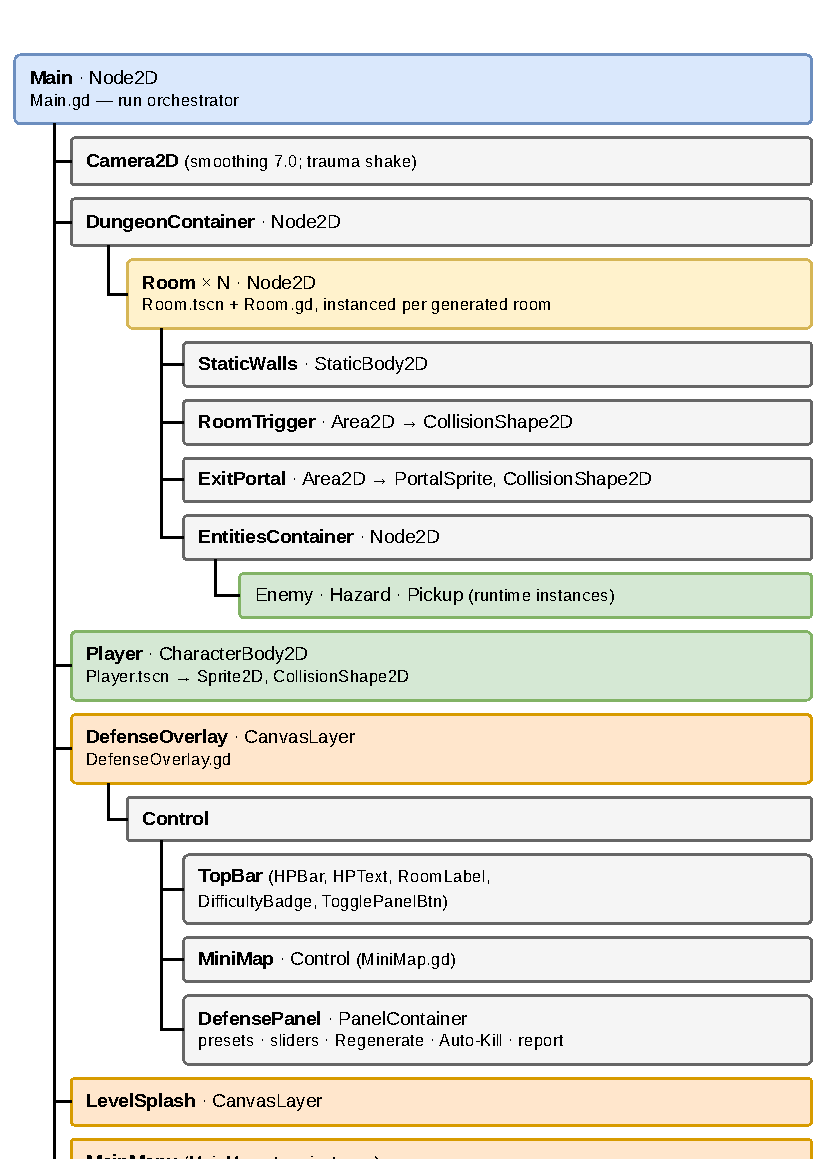
\includegraphics[width=0.65\textwidth]{ThesisFigs/fig_6_3_godot_scene_tree_hierarchy}
\caption{Godot 4.x Node Composition and Scene Tree Hierarchy}
\label{fig:godot_scene_tree}
\end{figure}

\section{Completed Features and Modules}
\label{sec:iter1_features}

\subsection{Visual Aesthetics Overhaul and Combat Juice}
Fulfilling the committee's mandate regarding visual quality:
\begin{itemize}
    \item \textbf{2D Pixel-Art Sprites:} Replaced procedural circles with top-down pixel-art assets ($64\times64$\,px single-frame sprites generated by a Pillow script; motion such as the walk wobble and projectile orientation is produced in code):
    \begin{itemize}
        \item \texttt{player.png}: Armored knight; the sword swing is drawn in code.
        \item \texttt{enemy\_crawler.png}: Demonic melee crawler with horns and red eyes.
        \item \texttt{enemy\_pyromancer.png}: Robed caster with a staff; the charge telegraph is a yellow ring drawn in code.
        \item \texttt{projectile\_fireball.png}: High-contrast fireball ($24\times24$\,px), rotated to its flight direction.
        \item \texttt{tile\_floor\_stone.png}: Stone flagstones, with separate floor tiles for start, hazard, treasure, and exit rooms.
    \end{itemize}
    \item \textbf{Camera Trauma Shake:} Integrated non-linear trauma screen shake (decay rate $3.6$\,s$^{-1}$) in \texttt{Main.gd}. Every player hit, hazard damage, or adversary elimination injects trauma ($T \leftarrow \min(T + \Delta, 1.0)$), producing a short, readable recoil.
    \item \textbf{Floating Combat Text (\texttt{DamageFloater.tscn}):} Created an animated numerical indicator that tweens upward with scale pop upon damage events: yellow for damage inflicted on enemies, crimson red for damage taken by the player, and emerald green for health potion restoration.
    \item \textbf{Typography Polish:} Integrated two Google Fonts (SIL Open Font License): \textbf{Cinzel} for atmospheric headers and badges, and \textbf{Inter} for HUD telemetry readouts.
\end{itemize}

\subsection{Multi-Archetype Combat Dynamics}
To eliminate combat monotony, we implemented two complementary enemy archetypes:
\begin{itemize}
    \item \textbf{Melee Crawler:} Chases the player directly upon entering aggro range ($240$\,px) at the PPO-controlled movement speed (default $125$\,px/s). Inflicts $20$ damage (default) per strike with a $0.8$\,s attack cooldown.
    \item \textbf{Ranged Pyromancer:} Maintains a tactical standoff band of $140$--$280$\,px, kiting backwards at $1.15\times$ speed when the player closes within $140$\,px. While its cooldown allows, it charges a telegraphed fireball with a $0.5$\,s yellow glow and then fires a projectile at $240$\,px/s along the direction to the player (default $18$ damage, i.e.\ $0.9\times$ the base enemy damage).
    \item \textbf{Player Dodge Roll / Dash:} Bound to the \texttt{Spacebar}, the player executes a high-speed dash ($0.2$\,s duration) with $0.26$\,s of invulnerability (the dash plus a $0.06$\,s grace period), governed by a $1.0$\,s cooldown bar on the HUD.
\end{itemize}

\subsection{5-Floor Cold-Start Calibration Protocol ($CR_0$ Mathematics)}
To avoid starting the adaptive phase from an arbitrary difficulty (the cold-start problem), \texttt{DifficultyManager.gd} executes a structured 5-floor calibration sequence with escalating difficulty parameter tiers:
\begin{enumerate}
    \item \textbf{Floor 1 (Novice Initiation):} 3 rooms, low adversary HP ($35$), minimal damage ($10$), $5\%$ traps.
    \item \textbf{Floor 2 (Swarm Reflex):} 4 rooms, more enemies per room ($\times0.9$ vs.\ $\times0.7$), mixed archetypes ($35\%$ Pyromancers), standard speed ($110$\,px/s), $15\%$ traps.
    \item \textbf{Floor 3 (Ranged Evasion \& Traps):} 4 rooms, Pyromancers only, high trap density ($38\%$), agile enemies ($135$\,px/s).
    \item \textbf{Floor 4 (Tactical Crucible):} 5 rooms, resilient adversaries (HP $70$, dmg $24$), $50\%$ traps.
    \item \textbf{Floor 5 (Apex Gauntlet):} 5 rooms, maximum stress test, high-speed adversaries ($175$\,px/s, dmg $30$), $65\%$ traps.
\end{enumerate}

At the exit of Floor 5, \texttt{TelemetryLogger.gd} calculates the non-uniform difficulty-weighted composite score:
\begin{equation}
\vec{w} = [1.0, \, 1.5, \, 2.0, \, 2.5, \, 3.0] \quad \left(\sum_{i=1}^5 w_i = 10.0\right)
\label{eq:weights}
\end{equation}
For each floor $i$, the engine evaluates:
\begin{align}
\text{Pace}_i &= \text{clamp}\left(1.0 - \frac{\text{sec\_per\_room}_i - 5.0}{12.0}, \, 0.0, \, 1.0\right) \\
\text{Survival}_i &= \begin{cases} 1.0 & \text{if } n_{\text{deaths}} = 0 \\ 0.5 & \text{if } n_{\text{deaths}} = 1 \\ 0.0 & \text{if } n_{\text{deaths}} \ge 2 \end{cases} \\
\text{Resistance}_i &= \text{clamp}\left(1.0 - \frac{\text{dmg\_taken}_i}{120.0}, \, 0.0, \, 1.0\right)
\end{align}
The Initial Combat Rating ($CR_0 \in [10, 95]$) is synthesized as:
\begin{equation}
CR_0 = \left(\frac{\sum w_i \cdot \text{Survival}_i}{\sum w_i} \cdot 40.0\right) + \left(\frac{\sum w_i \cdot \text{Resistance}_i}{\sum w_i} \cdot 35.0\right) + \left(\frac{\sum w_i \cdot \text{Pace}_i}{\sum w_i} \cdot 25.0\right)
\label{eq:cr0_formula}
\end{equation}
$CR_0$ is a human-readable summary shown to the player and evaluator. The policy is never given $CR_0$ itself: it was trained on raw per-floor signals, so the first adaptive observation $s_0$ is built from the same weighted calibration records on the training scales (Section~\ref{sec:obs_contract}):
\begin{equation}
\begin{aligned}
s_0[\text{time}] &= \frac{1}{\sum_i w_i}\sum_i w_i \, \text{clamp}\!\left(\frac{6\cdot\text{sec\_per\_room}_i}{90}\right),\\
s_0[\text{deaths}] &= \frac{1}{\sum_i w_i}\sum_i w_i \, \text{clamp}\!\left(\frac{n_{\text{deaths},i}}{3}\right),\\
s_0[\text{dmg}] &= \frac{1}{\sum_i w_i}\sum_i w_i \, \text{clamp}\!\left(\frac{\text{dmg\_taken}_i}{\text{max\_hp}}\right)
\end{aligned}
\label{eq:s0_seed}
\end{equation}
with the remaining five entries taken from the Floor 5 parameters and run depth. An earlier version passed $1-\overline{\text{Pace}}$, $1-\overline{\text{Survival}}$ and $1-\overline{\text{Resistance}}$ instead, which are on different scales from training (e.g., an on-target pace mapped to $0.21$ instead of $0.5$); this was corrected before submission (DEF-06) and is covered by test TC-02. Because the seed rests on only five floors, it is a starting estimate rather than an accurate measure of skill; the closed loop then adjusts from Floor 6 onwards.

\subsection{Static Non-Adaptive Roguelike Baseline Mode}
In \texttt{DefenseOverlay.gd}, the team integrated a live toggle button switching between:
\begin{itemize}
    \item \textbf{Mode: Adaptive Closed-Loop (PPO):} PPO dynamically balances encounter parameters based on live telemetry observations.
    \item \textbf{Mode: Static Baseline (Non-Adaptive):} PPO updates are bypassed; adversary health and damage grow deterministically by $8\%$ of the Intermediate preset value per floor (linear, not compounding), with all other parameters fixed. This is the non-adaptive comparison condition; a comparative evaluation against it is scheduled for FYP-1 Final.
\end{itemize}

\section{Technical Implementation Details and Code Artifacts}

\subsection{Pure-GDScript Neural Forward Pass (\texttt{PPOPolicy.gd})}
Listing~\ref{lst:ppo_predict} presents the core matrix multiplication and activation forward pass implemented in native GDScript.

\begin{lstlisting}[language=Python, caption={Native GDScript Forward Pass Implementation in \texttt{PPOPolicy.gd}}, label={lst:ppo_predict}]
func predict(obs: PackedFloat32Array) -> PackedFloat32Array:
    if not loaded:
        return _fallback_heuristic(obs)

    var x: Array = []
    for v in obs:
        x.append(v)

    for i in range(layers.size()):
        var layer: Dictionary = layers[i]
        var w: Array = layer["w"]   # shape [out_dim][in_dim]
        var b: Array = layer["b"]   # shape [out_dim]
        var y: Array = []
        y.resize(w.size())
        for o in range(w.size()):
            var s: float = b[o]
            var row: Array = w[o]
            for k in range(row.size()):
                s += float(row[k]) * float(x[k])
            y[o] = s
        var is_last := (i == layers.size() - 1)
        if not is_last:                    # tanh on hidden layers only
            for o in range(y.size()):
                y[o] = tanh(y[o])
        x = y

    # Output layer = Gaussian mean; clip to [-1, 1] exactly as
    # SB3's deterministic predict() did during training (DEF-07)
    var out := PackedFloat32Array()
    for v in x:
        out.append(clampf(v, -1.0, 1.0))
    return out
\end{lstlisting}

\subsection{Heuristic Fallback Mechanism}
Listing~\ref{lst:fallback} shows the rule-based fallback in \texttt{PPOPolicy.gd}, used when \texttt{policy\_weights.json} is missing or cannot be parsed so that the game stays playable.

\begin{lstlisting}[language=Python, caption={Deterministic Heuristic Fallback in \texttt{PPOPolicy.gd}}, label={lst:fallback}]
func _fallback_heuristic(obs: PackedFloat32Array) -> PackedFloat32Array:
    var norm_time: float = obs[0]
    var norm_deaths: float = obs[1]
    var norm_dmg_ratio: float = obs[2]
    var cur_hp: float = obs[3]
    var cur_dmg: float = obs[4]
    var cur_haz: float = obs[5]
    var cur_rooms: float = obs[6]

    # > 0: player did well -> escalate, < 0: player struggled -> ease off
    var performance_signal: float = (0.5 - norm_time) * 1.4 \
        - norm_deaths * 1.5 - norm_dmg_ratio * 0.8
    performance_signal = clampf(performance_signal, -1.0, 1.0)

    var step := 0.12   # per-level nudge, in normalized [-1, 1] units
    var out := PackedFloat32Array()
    out.append(clampf(cur_hp * 2.0 - 1.0 + performance_signal * step, -1.0, 1.0))
    out.append(clampf(cur_dmg * 2.0 - 1.0 + performance_signal * step, -1.0, 1.0))
    out.append(clampf(performance_signal * 0.5, -1.0, 1.0))   # enemy_speed
    out.append(clampf(performance_signal * 0.5, -1.0, 1.0))   # enemy_aggro
    out.append(clampf(cur_haz * 2.0 - 1.0 + performance_signal * step, -1.0, 1.0))
    out.append(clampf(performance_signal * 0.3, -1.0, 1.0))   # resource_scarcity
    out.append(clampf(cur_rooms * 2.0 - 1.0 + performance_signal * step, -1.0, 1.0))
    return out
\end{lstlisting}

\subsection{Ranged Pyromancer Projectile Instantiation}
In \texttt{Enemy.gd}, a Ranged Pyromancer that is within aggro range and off cooldown enters the \texttt{CHARGING} state for $0.5$\,s and then calls \texttt{shoot\_fireball()}:
\begin{lstlisting}[language=Python, caption={Telegraphed Fireball Spawning in \texttt{Enemy.gd}}, label={lst:enemy_attack}]
# in _process_pyromancer_ai(): telegraph, then fire
if is_charging:
    current_state = State.CHARGING
    charge_timer += delta
    move_velocity = -dir_to_player * 18.0       # hold ground while casting
    if charge_timer >= charge_duration:         # 0.5 s telegraph
        is_charging = false
        shoot_fireball(dir_to_player)
    return move_velocity

func shoot_fireball(target_dir: Vector2) -> void:
    attack_cooldown_timer = attack_rate
    if projectile_scene:
        var p = projectile_scene.instantiate()
        var spawn_pos = global_position + target_dir * 28.0
        get_parent().add_child(p)
        p.setup(target_dir, spawn_pos, attack_damage, 240.0)
        apply_knockback(-target_dir * 90.0)
\end{lstlisting}

\section{Tools, Frameworks and Technologies Used}
Table~\ref{tab:tech_stack} summarizes the technology stack employed during Iterations 1 and 2.

\begin{table}[!htbp]
\centering
\caption{FORGE Technology Stack and Infrastructure}
\label{tab:tech_stack}
\small
\begin{tabular}{p{0.25\textwidth}p{0.25\textwidth}p{0.45\textwidth}}
\toprule
\textbf{Layer / Domain} & \textbf{Technology} & \textbf{Role in FORGE Architecture} \\
\midrule
Game Engine & Godot 4.7.2 (development and CI) & Core 2D physics, tilemaps, node hierarchy, visual rendering. \\
In-Game Scripting & GDScript 2.0 & Engine logic and embedded neural forward pass. \\
Offline RL Training & Python 3.12 / SB3 & Gymnasium environment, PPO policy optimization, weight export. \\
Neural Framework & PyTorch $\ge 2.0$ & Multilayer Perceptron tensor operations and gradient calculations. \\
Continuous Integration & GitHub Actions & Headless Godot load check, reachability regression test, GDScript tests; Python lint and tests. \\
Version Control & Git / GitHub & Distributed source management, atomic commits, and release tagging. \\
Typography \& Assets & Google Fonts / Pixel Art & Cinzel, Inter typography; script-generated 2D dungeon sprites. \\
\bottomrule
\end{tabular}
\end{table}

\section{Demonstration Evidence}
The implemented system was validated through live gameplay sessions and headless test suites:
\begin{itemize}
    \item \textbf{Aesthetic Verification:} Pixel-art sprites render on the stone floor tiles without visible stutter in supervised play (frame times not yet logged). Trauma camera shake triggers visibly upon taking damage.
    \item \textbf{Tactical Evasion Evidence:} Spacebar dodge rolls reliably grant iframes, allowing players to roll through Pyromancer fireballs without sustaining damage.
    \item \textbf{Telemetry Verification:} The JSON telemetry file (\texttt{session\_telemetry.json}) logs cumulative damage taken and dealt, deaths, rooms cleared, kills, pickups and hazard hits; a headless test (TC-01) confirms exact damage values inside the real game scene. Before fix DEF-05, damage was not recorded (all 50 earlier snapshots show 0.0).
    \item \textbf{Defense Overlay Inspector:} Evaluators can press \texttt{Tab} in real-time to toggle between PPO Adaptive and Static Baseline modes, observe live parameter numbers, and adjust sliders dynamically.
\end{itemize}

\section{Iteration Outcome}
Iterations 1 and 2 delivered all planned Mid-1 features and addressed seven of the ten committee directives fully and three partially (Table~\ref{tab:action_register}). The prototype is a playable, visually polished 2D combat roguelike with a two-stage generator, connected by construction, and embedded RL difficulty conditioning. The main open technical issue is that the trained policy personalizes only part of its action space (Section~\ref{sec:policy_eval}).
